Step 1: Construct the Augmented Matrix
\begin{align}
\myvec{
8&5&9\\
3&2&4
}
\end{align}

Step 2: Perform row opertions to get a Row Echelon form\\
\begin{align}
\myvec{
8&5&9\\
3&2&4 
}
\xleftrightarrow{ R_2\rightarrow 8 R_2-3 R_1}
\myvec{
8&5&9\\
0&1&5
}\\
\myvec{
8&5&9\\
0&1&5
}
\xleftrightarrow{ R_1\rightarrow R_1- 5 R_2}
\myvec{
8&0& -16\\
0&1&5 
}\\
\myvec{
8&0& -16\\
0&1&5 
}
\xleftrightarrow{ R_1\rightarrow \frac{R_1}{8}}
\myvec{
1&0&-2\\
0&1&5
}
\end{align}
Above final matrix is in the reduced Echelon form and from this matrix we get the solution. Last column represents the solution of the given linear equation.
Hence the solution is: {\myvec{-2\\ 5}}
See Fig. \ref{fig:plotsolutions/line_plane/22/}

\begin{figure}[!ht]
\centering
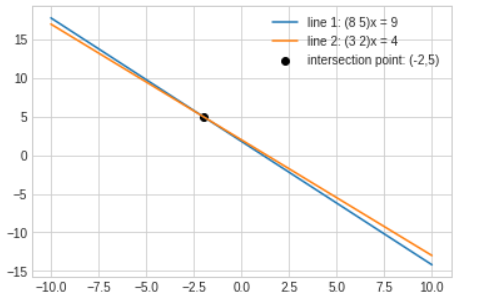
\includegraphics[width=\columnwidth]{./solutions/line_plane/22/plot.png}
\caption{Linear equations plot generated using python}
\label{fig:plotsolutions/line_plane/22/}
\end{figure}


